\section{Architektur}
tbd

\subsection{Architekturübersicht}
Alter Stand tbd
Nach der Vorstellung der verwendeten Technologien beschreibt dieser Abschnitt den Aufbau der Gesamtarchitektur. Für das Lesen der Arbeit stellt die Übersicht eine Orientierungshilfe dar, um die technische Gliederung der Lösung von Beginn an nachvollziehbar zu machen.

Die Lösung ist modular aufgebaut und besteht aus zwei getrennten Extensions. Eine ist für das virtuelle Filesystem zuständig, die andere für die Editorunterstützung. Der Editor ist die Schnittstelle, über die die Editorunterstützung auf die Inhalte des virtuellen Filesystem zugreift.

...tbd


\begin{figure}[H]
  \centering
  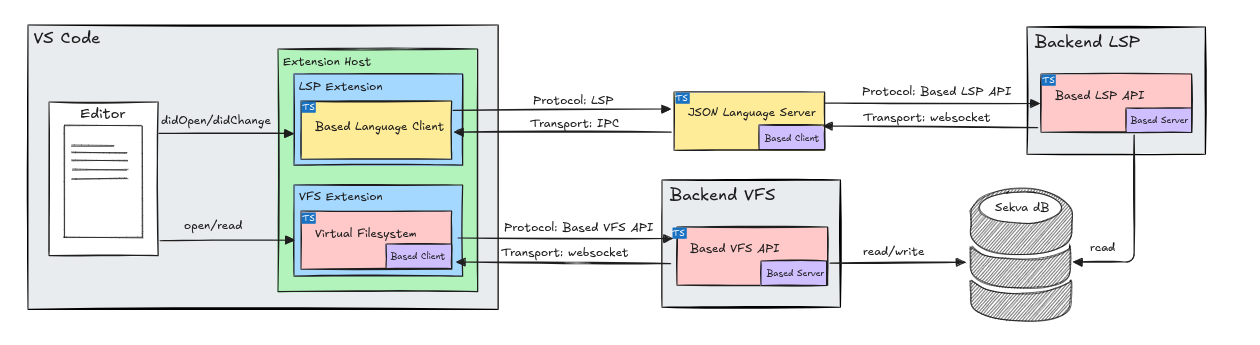
\includegraphics[width=\linewidth]{Arch.png}
  \caption{Architekturübersicht der implementierten Lösung}
  \label{fig:arch_modell}
\end{figure}
